\section{Проектирование архитектуры распределённой платформы}

\subsection{Архитектурные принципы}

Архитектура платформы строится как набор автономных микросервисов с разделением ответственности по этапам жизненного цикла уведомления \cite{newman_microservices,richardson_patterns,kleppmann_ddia}. Основная граница проходит между командным контуром, который принимает и фиксирует уведомительное событие, и фоновым контуром, который выполняет запуск доставки, канальную обработку и запись истории.

В качестве базовых принципов приняты:
\begin{enumerate}
    \item разделение командного и асинхронного контуров;
    \item локальная транзакционность внутри одного сервиса без распределённых транзакций;
    \item сквозная идемпотентность на уровне команд, запусков доставки и событийного обмена;
    \item сохранение промежуточных состояний в собственных хранилищах сервисных контуров;
    \item централизованная проверка профиля получателя;
    \item наблюдаемость всех основных переходов обработки.
\end{enumerate}

Командный контур использует gRPC и protobuf-контракты для операций, результат которых нужен вызывающей системе сразу: создание уведомительного события, чтение состояния, запуск доставки, чтение истории. Фоновый контур использует Kafka, чтобы вынести фактическую доставку из критического пути клиентского запроса и отделить приём команд от работы sender-сервисов \cite{grpc_docs,kafka_docs,nygard_releaseit}.

Внешние границы платформы и её интеграции показаны на рисунке~\ref{fig:arch-system-context-structurizr}.

\begin{figure}[H]
    \centering
    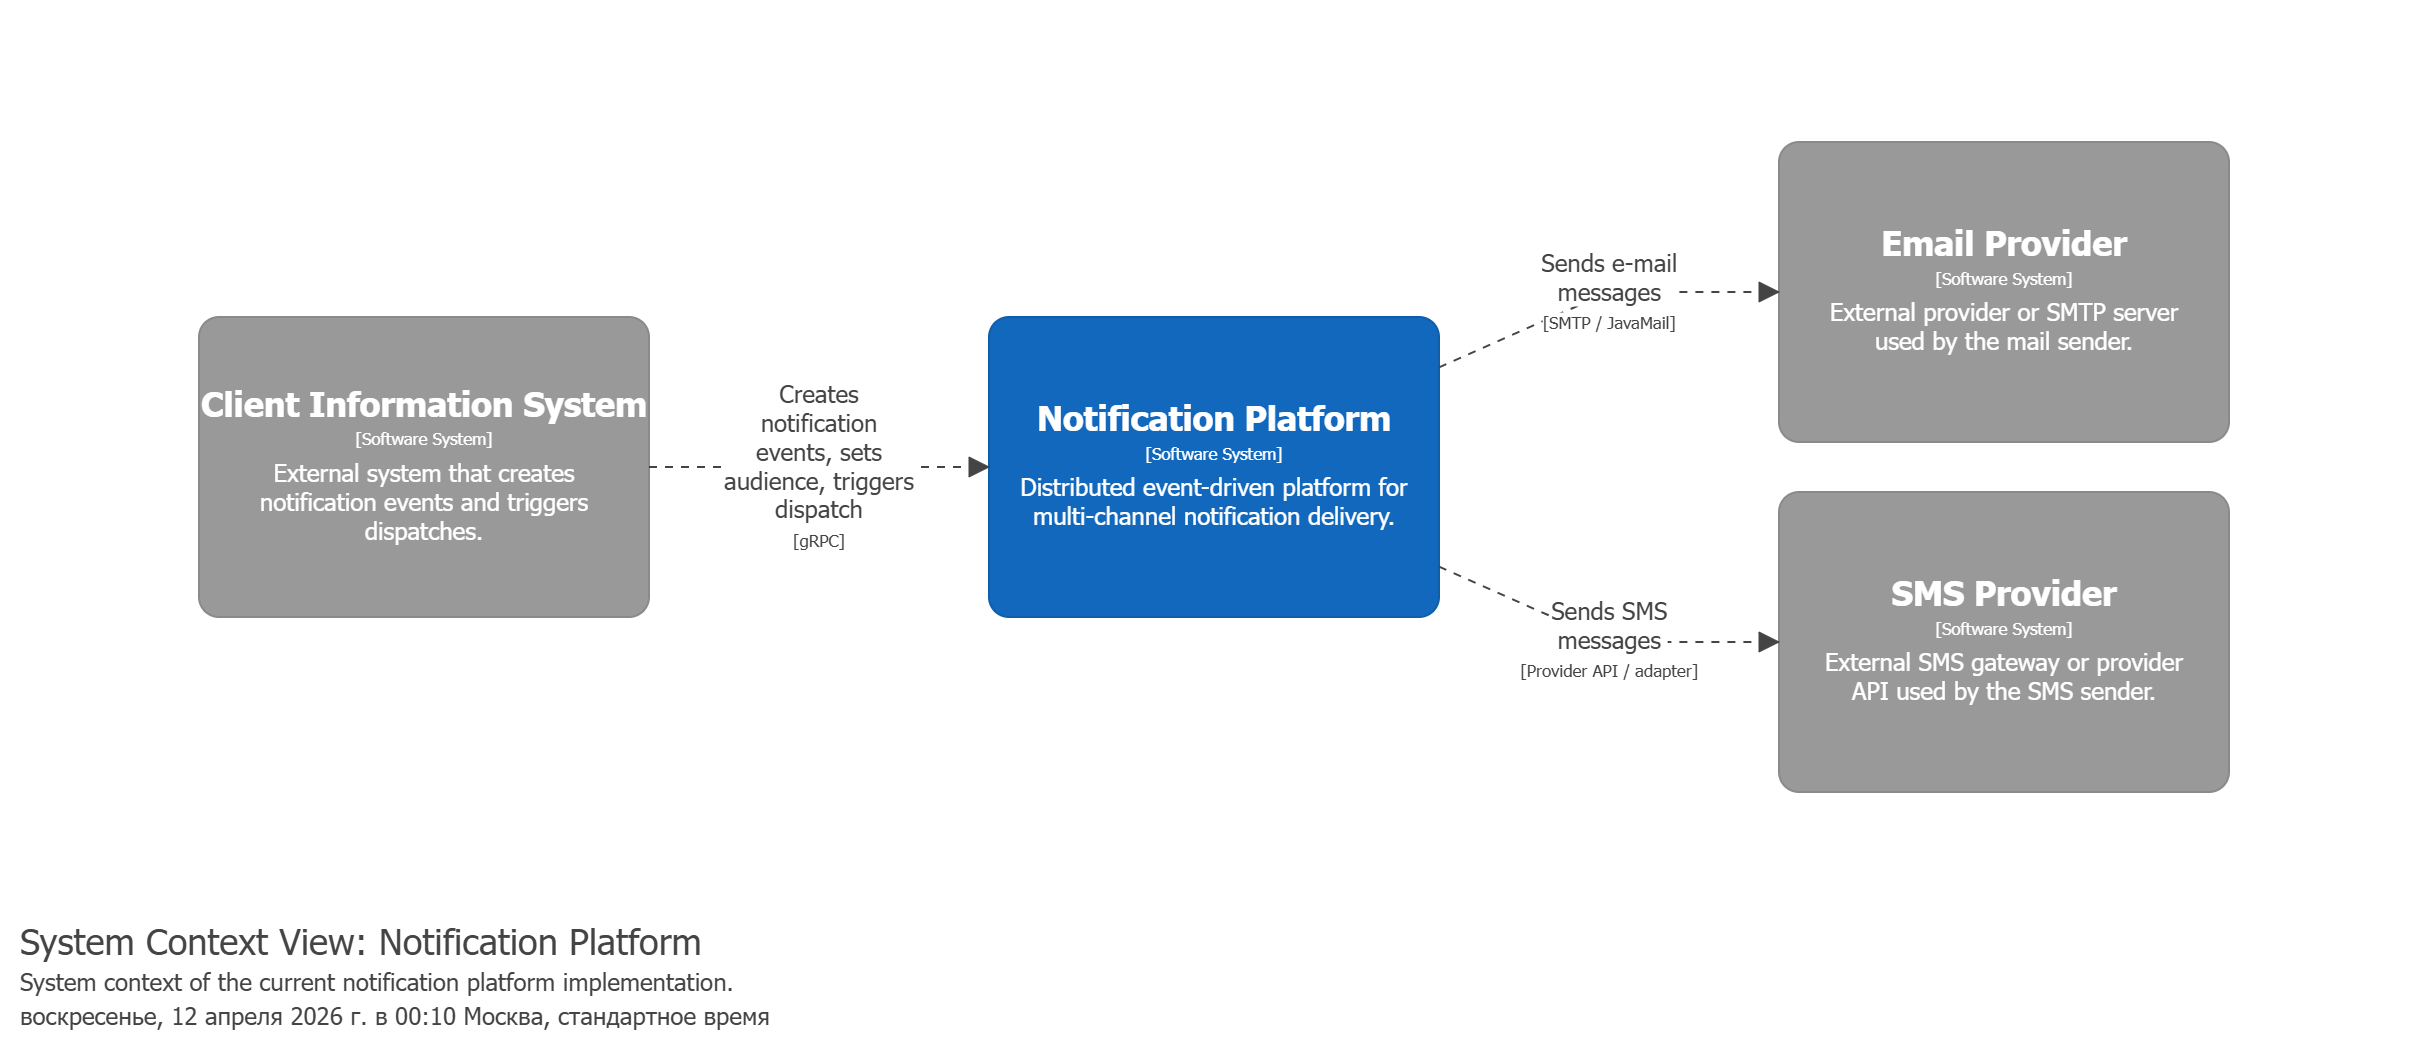
\includegraphics[width=\textwidth]{inc/structurizr-system-context.png}
    \caption{Системный контекст платформы уведомлений}
    \label{fig:arch-system-context-structurizr}
\end{figure}

Системный контекст нужен не как обзор компонентов, а как фиксация границы ответственности платформы. Клиентская система взаимодействует только с командным контуром, а внешние email- и SMS-провайдеры доступны только sender-сервисам. Это исключает прямую связность пользовательского запроса с внешним каналом связи и локализует риски деградации на стороне фоновой обработки.

\subsection{Контейнерная декомпозиция и границы ответственности}

Контейнерная декомпозиция определяется не только набором сервисов, но и владением данными. Каждый сервис, владеющий собственным состоянием, использует отдельное хранилище и не обращается напрямую к данным другого сервиса. Межсервисный обмен выполняется через gRPC и Kafka, а не через прямое чтение чужих таблиц или коллекций.

\begin{figure}[H]
    \centering
    \footnotesize
    \setlength{\tabcolsep}{4pt}
    \renewcommand{\arraystretch}{1.3}
    \begin{tabular}{ccc}
        \fbox{\parbox[c][1.6cm][c]{0.24\textwidth}{\centering Клиентская\\информационная система}} &
        $\rightarrow$ &
        \fbox{\parbox[c][1.6cm][c]{0.24\textwidth}{\centering Notification Facade\\gRPC-команды, аудитория, запуск доставки}} \\
        & & \fbox{\parbox[c][1.3cm][c]{0.24\textwidth}{\centering Facade PostgreSQL\\notification\_event, audience, dispatch, outbox}} \\[4pt]
        \fbox{\parbox[c][1.5cm][c]{0.24\textwidth}{\centering Template Registry\\версии шаблонов, предварительный рендеринг}} &
        \fbox{\parbox[c][1.5cm][c]{0.22\textwidth}{\centering Kafka\\notification.facade.events\\notification.mail.dispatches\\notification.mail.scheduled\\notification.sms.dispatches\\notification.delivery-statuses}} &
        \fbox{\parbox[c][1.5cm][c]{0.24\textwidth}{\centering Profile Consent\\проверка профиля получателя}} \\
        \fbox{\parbox[c][1.2cm][c]{0.24\textwidth}{\centering MongoDB Templates}} & &
        \fbox{\parbox[c][1.2cm][c]{0.24\textwidth}{\centering Redis Recipient Profiles}} \\[4pt]
        \fbox{\parbox[c][1.5cm][c]{0.24\textwidth}{\centering Scheduler Delivery\\отложенный запуск}} &
        \fbox{\parbox[c][1.5cm][c]{0.24\textwidth}{\centering Notification Mail Sender\\email-обработка, retry, status}} &
        \fbox{\parbox[c][1.5cm][c]{0.24\textwidth}{\centering Notification SMS Sender\\SMS-обработка, retry, status}} \\
        \fbox{\parbox[c][1.2cm][c]{0.24\textwidth}{\centering Scheduler PostgreSQL}} &
        \fbox{\parbox[c][1.2cm][c]{0.24\textwidth}{\centering Mail PostgreSQL}} &
        \fbox{\parbox[c][1.2cm][c]{0.24\textwidth}{\centering SMS PostgreSQL}} \\[4pt]
        \multicolumn{3}{c}{
            \fbox{\parbox[c][1.5cm][c]{0.30\textwidth}{\centering History Writer\\история статусов, сводки}}
            \hspace{0.02\textwidth}
            \fbox{\parbox[c][1.2cm][c]{0.20\textwidth}{\centering History PostgreSQL}}
        } \\[4pt]
        \multicolumn{3}{c}{
            \fbox{\parbox[c][1.1cm][c]{0.26\textwidth}{\centering Prometheus / Grafana}}
            \hspace{0.02\textwidth}
            \fbox{\parbox[c][1.1cm][c]{0.22\textwidth}{\centering SMTP /\\email-провайдер}}
            \hspace{0.02\textwidth}
            \fbox{\parbox[c][1.1cm][c]{0.22\textwidth}{\centering SMS-провайдер}}
        }
    \end{tabular}
    \caption{Контейнерная архитектура платформы уведомлений с разделением хранилищ по сервисным контурам}
    \label{fig:arch-containers-owned-storage}
\end{figure}

Рисунок~\ref{fig:arch-containers-owned-storage} отражает не только сервисы, но и владение данными. Notification Facade, Scheduler Delivery, Notification Mail Sender, Notification SMS Sender и History Writer используют отдельные PostgreSQL-хранилища. Template Registry владеет MongoDB-хранилищем шаблонов, а Profile Consent владеет Redis-хранилищем профилей получателей. Такое разделение исключает превращение базы данных в общий интеграционный слой и принуждает сервисы обмениваться данными только через контракт владельца.

\subsection{Верхнеуровневая модель данных и сервисных границ}

Архитектурная модель опирается на четыре уровня сущностей:
\begin{enumerate}
    \item уведомительное событие как описание намерения;
    \item запуск доставки как экземпляр исполнения события;
    \item канальная доставка как обработка пары «получатель --- канал»;
    \item история доставки как журнал и агрегированное представление итогов.
\end{enumerate}

Такое разделение определяет границы сервисов. Фасад владеет событием и запуском доставки, sender-сервисы владеют канальной доставкой и попытками отправки, history-writer владеет фактами изменения статуса. Template Registry и Profile Consent вынесены в отдельные контуры, поскольку они обслуживают сразу несколько этапов обработки и несколько каналов.

Состав контейнеров и их роль приведены в таблице~\ref{tab:architecture-containers}.

\begin{table}[H]
    \centering
    \footnotesize
    \renewcommand{\arraystretch}{1.15}
    \caption{Контейнеры и их ответственность}
    \label{tab:architecture-containers}
    \begin{tabular}{|L{0.24\textwidth}|L{0.38\textwidth}|L{0.25\textwidth}|}
        \hline
        \textbf{Контейнер} & \textbf{Ответственность} & \textbf{Собственное хранилище} \\
        \hline
        Notification Facade & Приём gRPC-команд, управление событиями, аудиторией и запусками доставки, публикация в Kafka. & Facade PostgreSQL \\
        \hline
        Template Registry & Хранение шаблонов, версий и канальных представлений, RenderPreview. & MongoDB Templates \\
        \hline
        Profile Consent & Выдача профиля получателя, разрешений каналов и адресных атрибутов. & Redis Recipient Profiles \\
        \hline
        Scheduler Delivery & Контур отложенной публикации запусков доставки. & Scheduler PostgreSQL \\
        \hline
        Notification Mail Sender & Обработка email-запусков, попытки отправки, retry и публикация статусов. & Mail PostgreSQL \\
        \hline
        Notification SMS Sender & Обработка SMS-запусков, попытки отправки, retry и публикация статусов. & SMS PostgreSQL \\
        \hline
        History Writer & Приём статусных событий, запись истории и формирование сводок. & History PostgreSQL \\
        \hline
        Kafka & Событийный обмен между сервисами и буферизация фоновой обработки. & Не применимо \\
        \hline
        Prometheus, Grafana & Наблюдаемость и контроль эксплуатационных показателей. & Метрики сервисов и Kafka-клиентов \\
        \hline
    \end{tabular}
\end{table}

\subsection{Верхнеуровневые потоки данных}

\subsubsection{Поток приёма команды и регистрации события}

Приём пользовательской команды выполняется в синхронном контуре. Notification Facade валидирует запрос, проверяет ключ идемпотентности, сохраняет уведомительное событие, аудиторию и запись outbox. Только после этого событие публикуется в Kafka для дальнейшей обработки.

Сценарий взаимодействий показан на рисунке~\ref{fig:arch-create-event-flow-structurizr}.

\begin{figure}[H]
    \centering
    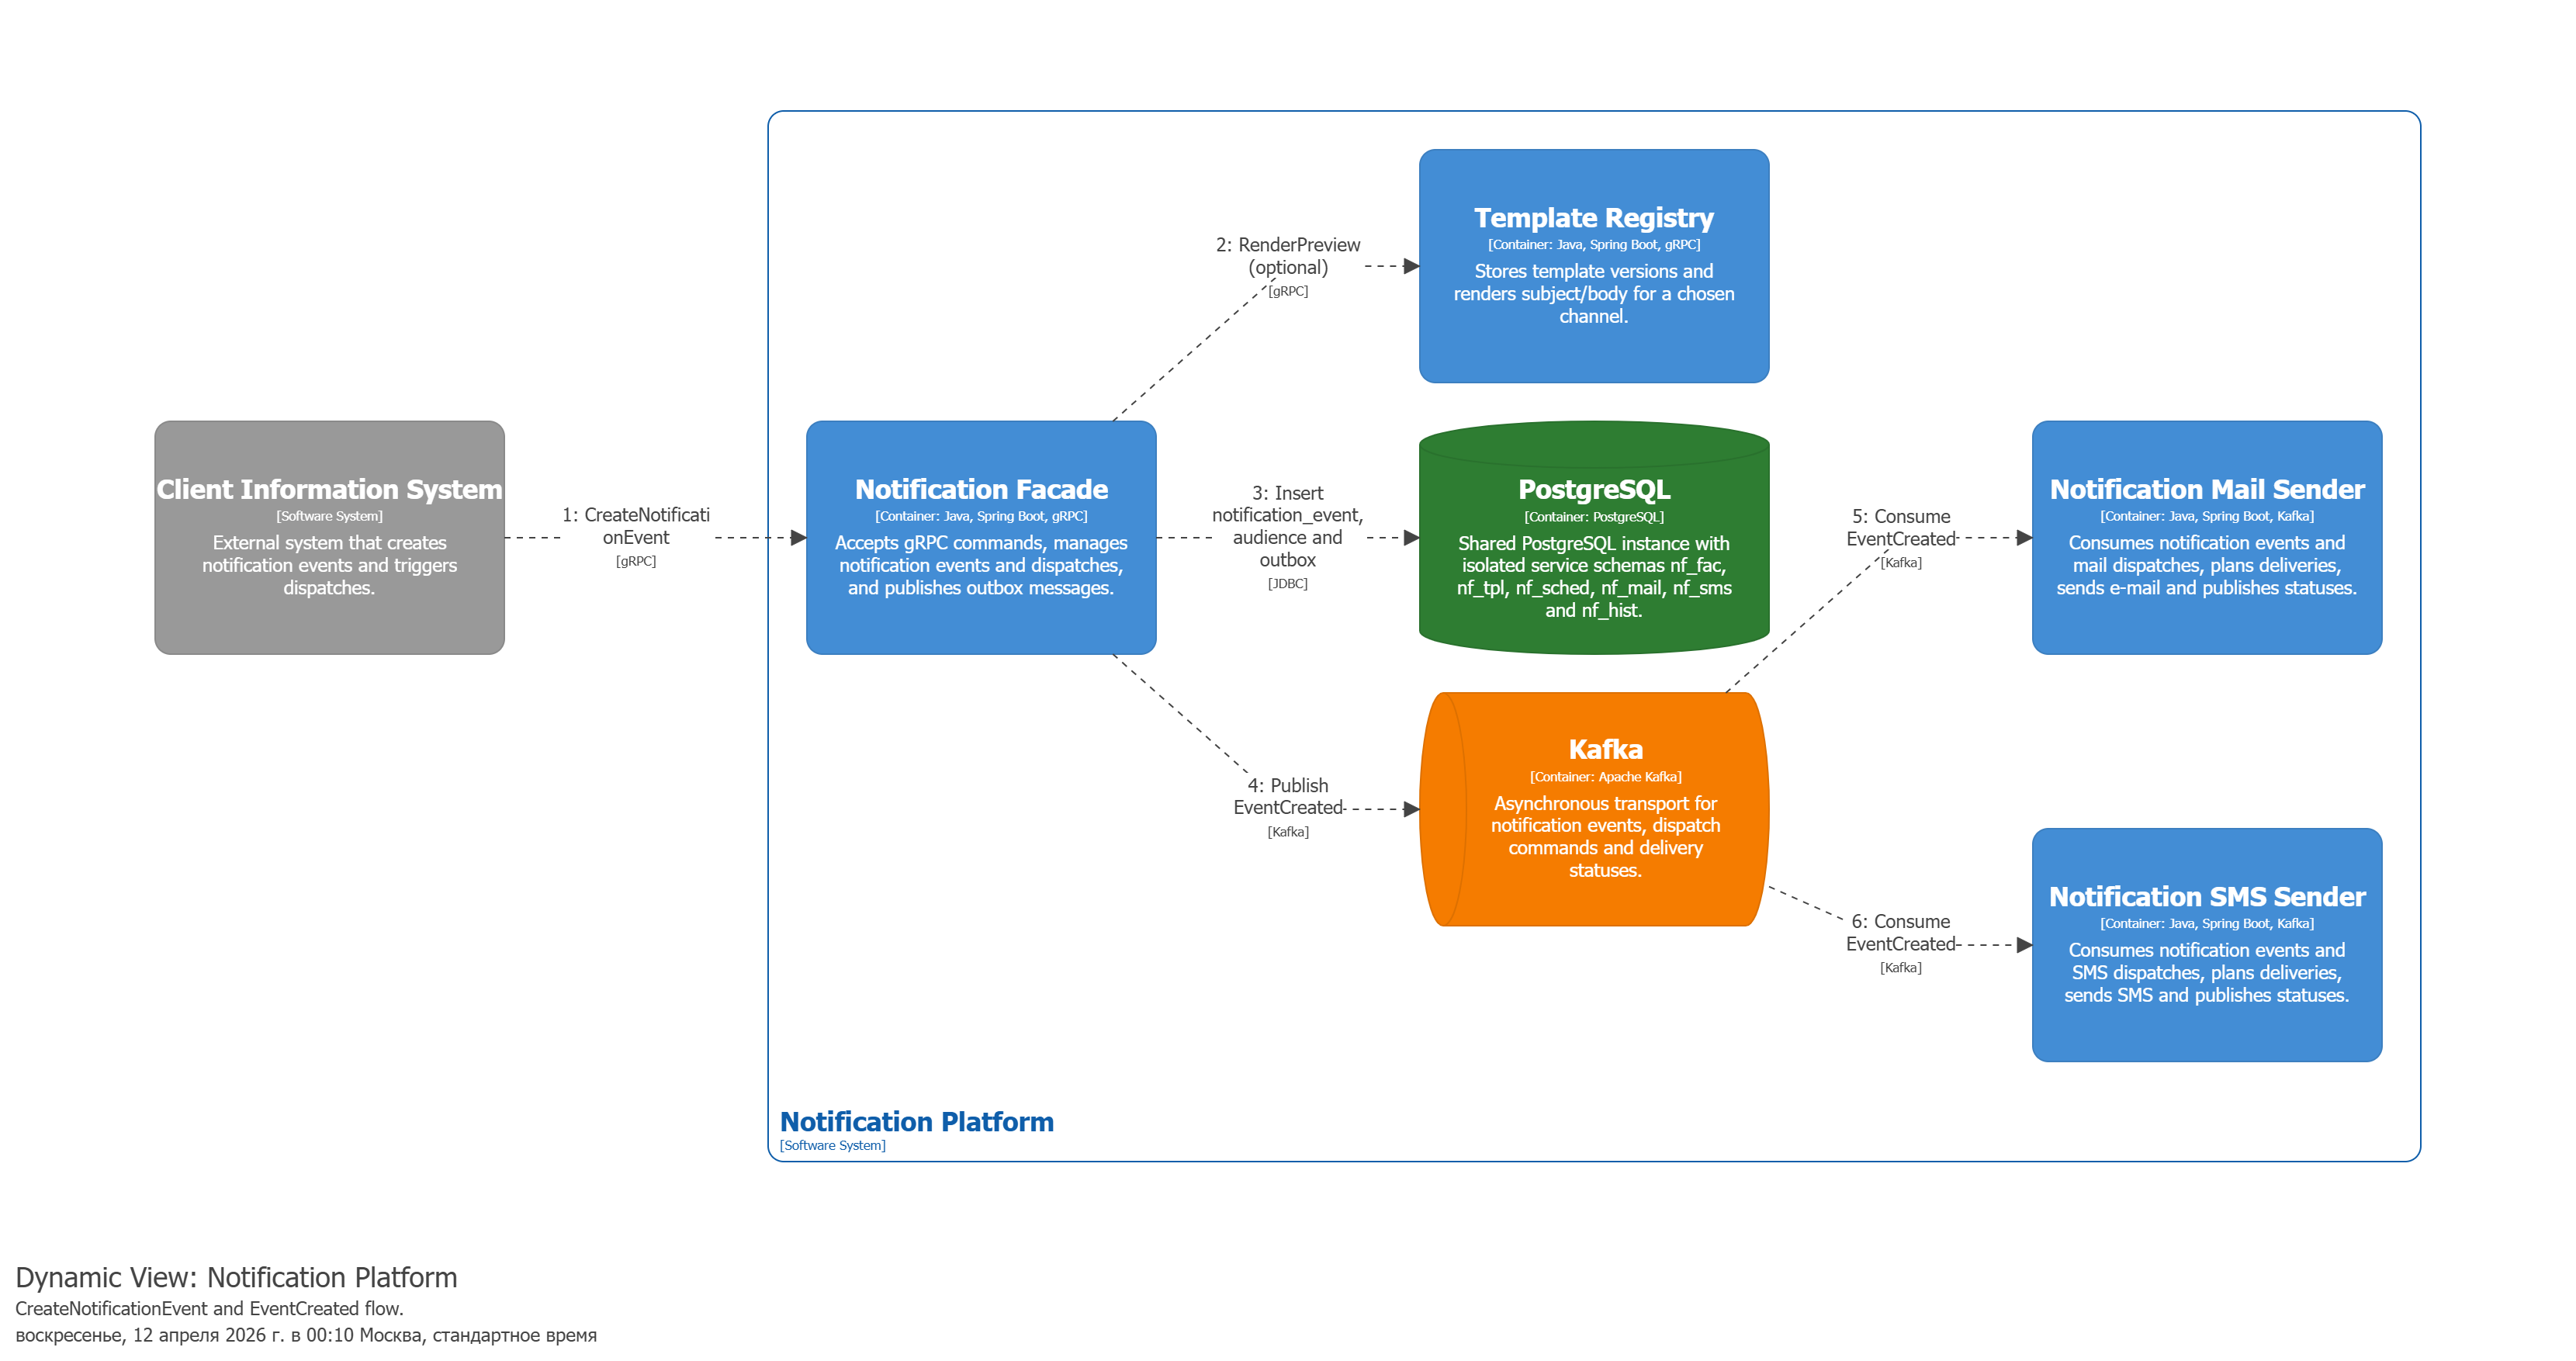
\includegraphics[width=\textwidth]{inc/structurizr-create-event-flow.png}
    \caption{Динамический поток регистрации события и передачи в событийный контур}
    \label{fig:arch-create-event-flow-structurizr}
\end{figure}

Рисунок~\ref{fig:arch-create-event-flow-structurizr} нужен для фиксации самой чувствительной точки архитектуры: перехода от синхронной команды к фоновому контуру. Именно здесь определяется, будет ли принятая команда потеряна при сбое сервиса между записью в базу и публикацией в брокер. В выбранной архитектуре этот риск закрывается локальной транзакцией и transactional outbox.

\subsubsection{Поток запуска доставки}

Запуск доставки отделён от этапа приёма команды. Такое решение даёт три практических эффекта:
\begin{enumerate}
    \item запуск можно выполнить сразу или по расписанию без изменения самой модели события;
    \item повторный запуск допустим без пересоздания уведомительного события;
    \item сбой канального контура не влияет на уже завершённый клиентский запрос.
\end{enumerate}

\subsubsection{Поток отложенной доставки}

Отложенная доставка вынесена в самостоятельный контур Scheduler Delivery. Фасад публикует запуск в отдельный scheduled-топик, планировщик сохраняет задачу в собственном PostgreSQL-хранилище и после наступления планового времени переводит её в рабочий Kafka-топик. Хранение отложенных задач в отдельном сервисе исключает зависимость от таймеров в памяти конкретного экземпляра приложения.

\subsubsection{Поток канальной обработки и истории}

Mail Sender и SMS Sender потребляют свои рабочие топики независимо друг от друга. Перед фактической отправкой sender-сервис обращается к profile-consent, получает решение по получателю и либо выполняет отправку, либо фиксирует пропуск как доменный результат обработки. После завершения попытки sender публикует статусное событие, которое history-writer записывает в собственное хранилище и агрегирует для запросов чтения.

\subsection{Kafka-архитектура событийного контура}

Kafka используется как базовый транспорт асинхронного обмена между контурами:
\begin{enumerate}
    \item поток событий жизненного цикла уведомления;
    \item потоки рабочих запусков по каналам;
    \item поток отложенных email-запусков;
    \item поток статусных событий доставки.
\end{enumerate}

Ключевые топики текущей архитектуры приведены в таблице~\ref{tab:kafka-architecture-topics}.

\begin{table}[h]
    \centering
    \footnotesize
    \renewcommand{\arraystretch}{1.15}
    \caption{Kafka-топики и их назначение}
    \label{tab:kafka-architecture-topics}
    \begin{tabular}{|L{0.34\textwidth}|L{0.52\textwidth}|}
        \hline
        \textbf{Топик} & \textbf{Назначение} \\
        \hline
        \seqsplit{notification.facade.events} & События жизненного цикла уведомления, публикуемые фасадом для дальнейшей канальной обработки. \\
        \hline
        \seqsplit{notification.mail.dispatches} & Рабочие команды на email-доставку. \\
        \hline
        \seqsplit{notification.mail.scheduled} & Отложенные email-команды, которые сначала обрабатывает Scheduler Delivery. \\
        \hline
        \seqsplit{notification.sms.dispatches} & Рабочие команды на SMS-доставку. \\
        \hline
        \seqsplit{notification.delivery-statuses} & Итоговые статусы email- и SMS-доставки, поступающие в history-writer. \\
        \hline
    \end{tabular}
\end{table}

Таблица~\ref{tab:kafka-architecture-topics} показывает, что Kafka используется не как внешний интеграционный шлюз, а как внутренний транспорт для нескольких независимых стадий обработки. Отдельные рабочие топики по каналам позволяют масштабировать sender-сервисы независимо и не смешивать email- и SMS-обработку в одном consumer-контуре.

\subsubsection{Маршрут событийного потока}

Маршрут обработки в Kafka-контуре может быть представлен как последовательность доменных шагов:
\begin{enumerate}
    \item фасад публикует событие жизненного цикла уведомления в notification.facade.events;
    \item фасад формирует каналоспецифичный запуск и публикует его в notification.mail.dispatches или notification.sms.dispatches;
    \item при отложенной отправке запуск сначала попадает в notification.mail.scheduled, затем планировщик переносит его в рабочий топик;
    \item канальные обработчики публикуют итог в notification.delivery-statuses;
    \item сервис истории консолидирует статусные события в агрегированное представление получателя.
\end{enumerate}

\subsection{Механизмы надёжности на архитектурном уровне}

Надёжность обеспечивается сочетанием архитектурных механизмов:
\begin{enumerate}
    \item transactional outbox в фасаде и sender-сервисах для согласования доменного изменения и публикации интеграционного сообщения;
    \item transactional inbox в канальных обработчиках для регистрации входящего Kafka-сообщения перед бизнес-обработкой;
    \item idempotency key и уникальные ограничения для повторных команд и повторной доставки сообщения брокером;
    \item retry для временных ошибок и статусная модель для окончательных ошибок;
    \item history-writer как контур накопления фактов изменения статуса.
\end{enumerate}

Эта схема соответствует модели at-least-once доставки и управляемой eventual consistency между сервисами \cite{kafka_docs,richardson_patterns}. Дубликаты в транспортном слое допускаются, но подавляются на уровне приложения ключами идемпотентности, входящими журналами и уникальными ограничениями.

\subsection{Архитектура профиля получателя}

Профиль получателя выделен в отдельный сервисный контур. Profile Consent является единственной точкой доступа к Redis-хранилищу профилей получателей. Канальные сервисы не обращаются к Redis напрямую, а получают решение о допустимости доставки через сервисный контракт profile-consent.

На архитектурном уровне профиль включает:
\begin{enumerate}
    \item активность получателя;
    \item разрешения и ограничения по каналам;
    \item адресные данные, необходимые для email и SMS;
    \item технические атрибуты актуальности профиля.
\end{enumerate}

\subsection{Архитектура шаблонного контура}

Template Registry является единственным владельцем MongoDB-хранилища шаблонов. Остальные сервисы не обращаются к MongoDB напрямую и получают шаблонное содержимое только через сервисный контракт template-registry.

Выбор документоориентированной модели обусловлен структурой предметной сущности. Шаблон включает метаданные, активную версию и несколько канальных представлений, которые в типовом сценарии читаются совместно. Хранение этих данных в одном документе уменьшает число операций чтения при RenderPreview и при выборе активной версии для отправки \cite{mongodb_docs}.

\subsection{Архитектура наблюдаемости}

Наблюдаемость проектируется как обязательная часть архитектуры. Каждый сервис экспортирует метрики, достаточные для восстановления маршрута от входной команды до записи статуса в историю. Наиболее значимыми для этой платформы являются четыре группы метрик:
\begin{enumerate}
    \item gRPC server metrics командного контура;
    \item Kafka producer metrics на публикации событий и статусных сообщений;
    \item Kafka listener metrics на канальной обработке и в history-writer;
    \item JVM и process metrics для оценки ресурсных ограничений.
\end{enumerate}

Такой набор нужен не для общего мониторинга инфраструктуры, а для диагностики разрыва маршрута обработки: принят ли запрос, опубликовано ли событие, дошло ли оно до sender-сервиса и записан ли итоговый статус \cite{spring_boot_docs,kafka_docs}.

\subsection{Безопасность}

В пределах работы безопасность рассматривается на уровне сервисных границ и владения данными. Прикладной сервис не читает чужое хранилище напрямую, а использует только контракт владельца. Это уменьшает площадь непреднамеренного воздействия, упрощает разграничение ответственности и исключает зависимость бизнес-логики от внутренней схемы чужого хранилища.

Выбранная архитектура задаёт основу реализации: gRPC используется для командного контура, Kafka --- для фоновой обработки, а сохранность и повторяемость обработки обеспечиваются outbox/inbox, идемпотентностью и историей статусов.
